\documentclass{article}

% if you need to pass options to natbib, use, e.g.:
%     \PassOptionsToPackage{numbers, compress}{natbib}
% before loading neurips_2020
\PassOptionsToPackage{sort,numbers}{natbib}
% ready for submission
 \usepackage{neurips_2020}
 \usepackage{amssymb}

% to compile a preprint version, e.g., for submission to arXiv, add add the
% [preprint] option:
 %    \usepackage[preprint]{neurips_2020}

% to compile a camera-ready version, add the [final] option, e.g.:
%     \usepackage[final]{neurips_2020}

% to avoid loading the natbib package, add option nonatbib:
     %\usepackage[nonatbib]{neurips_2020}

\usepackage[utf8]{inputenc} % allow utf-8 input
\usepackage[T1]{fontenc}    % use 8-bit T1 fonts
\usepackage{hyperref}       % hyperlinks
\usepackage{url}            % simple URL typesetting
\usepackage{booktabs}       % professional-quality tables
\usepackage{amsfonts}       % blackboard math symbols
\usepackage{nicefrac}       % compact symbols for 1/2, etc.
\usepackage{microtype}      % microtypography


\usepackage{graphicx}
\usepackage{subfig}
\usepackage{amsmath}
\usepackage{algorithm}
\usepackage{algorithmic}



\title{Reflexive Reinforcement Learning: Supplementary Material}

% The \author macro works with any number of authors. There are two commands
% used to separate the names and addresses of multiple authors: \And and \AND.
%
% Using \And between authors leaves it to LaTeX to determine where to break the
% lines. Using \AND forces a line break at that point. So, if LaTeX puts 3 of 4
% authors names on the first line, and the last on the second line, try using
% \AND instead of \And before the third author name.

\author{
  B. I. Lyons \quad J. Michael Herrmann \\
  \\
  Institute for Perception, Action and Behaviour\\
  University of Edinburgh\\
  United Kingdom, EH8 9AB \\
  %\texttt{\{Billy.Lyons, Michael.Herrmann\}@ed.ac.uk} \\
}

\begin{document}

\centerline{\LARGE Reflexive Reinforcement Learning}
\medskip
\centerline{\large \rule[1mm]{1.1cm}{0.02cm} \quad Supplementary Material \quad \rule[1mm]{1.1cm}{0.02cm}}
\setcounter{section}{0}
\renewcommand\thesection{\Alph{section}}

\section{Reflexive Reinforcement Learning (RRL)}

\subsection{Inverse Reinforcement Learning (IRL)}

The self-generated rewards in reflexive reinforcement learning are expected to be 
self-consistently recoverable by inverse reinforcement learning, i.e.~the extracted reward 
distribution matches the initial rewards up to scale for a known original 
discount factor $\gamma$. %This has number of consequences for the RRL 
If $\gamma$ is not known, further ambiguities arise as any exponentially smoothed 
version of the original reward distribution is also a solution, such that a fixed environment-based 
choice of $\gamma$ is preferable.
%consider e.g.~the one-dimensional example, $r_0(x) = {\gamma_0}^{-1} \exp \left(- |x - x_0|/\gamma_0\right)$ for $x\in\mathbb{R}$ and a single goal state $x_0$.  

\subsection{Numerical stability}

The value of $\gamma$ has an obvious effect on the IRL solubility: For $\gamma\lessapprox 1$,  the stability of the inverse equations drop such that the quality of any finite-time 
estimation of the action-induced 
transitions will not be sufficient to solve the IRL problem.
Likewise, the numerical stability can also suffer from ambiguous reward configuration, such as 
the smoothening of reward distributions. This may
be useful to guide an agent gradually to a particular goal, but this would require 
precise goal-related prior information which is not assumed in a primarily exploratory problem setting. 

\subsection{Noise level}
The noise level is also a critical parameter in RRL. If the noise is high then a thorough 
exploration is possible, but less reward-related information is available to the IRL stage.
For small noise, the agent will slowly converge such that 
the reward-related information is not precise. The goal of RRL is to maximise the reward-related 
information flow.

\subsection{Maximum entropy IRL}

A single rewarded state would be easiest in the sense of numerical stability, but the success of
maximum entropy approaches~\cite{ziebart2008maximum} can serve as an argument for more general 
reward distributions such that the maximum entropy assumption is a-priorily correct.
In adversarial scenarios~\cite{finn2016connection} can provide the guidance 
necessary to generate the primal exploration schemes.

\subsection{Markovianity}

Markovianity can be guaranteed in the trivial case of information states, i.e.~if all previous state-actions pairs are  included in an exponentially large state space. In general, the requirement of Markovianity restricts somewhat the generality of RRL, and obviously
if the primal RL does not converge because of the non-Markovianity of the dynamics, then also IRL is bound to fail. This does not mean that a meaningful application of RRL always presupposes Markovianity.
 Indeed, RRL can be used to reduce the adverse effects of non-Markovianity, which proves advantageous, e.g., if the agent does not have full information about the state. 
In this case, the reward can be used to encourage state transitions that have observable consequences and that can be mapped to unique internal states which clearly helps to recover the reward signal in IRL.  


\subsection{Continuous States and Actions}

Introduction of a representation of policy and value function in terms of suitable chosen 
basis functions can improve the convergence rate, which holds both for primal RL and inverse RL.
While relations between the representations of policy and value function have been 
studied~\cite{kakade2002natural,sutton2000policy} the relation between RL and IRL is less 
understood, although usually the same representation can be used in either case. Thus, 
if the functional representation is known, then no additional problem arises in RRL in this 
respect.

In RRL the choice of a system of basis functions is obvious if taken jointly with the decision on 
the primal reward distribution: A function system is preferable if it represents perfectly 
the value function arising from the primal rewards. In addition, sparsity and 
low computational complexity are clearly beneficial. 

Using and finding symmetries~\cite{Ravindran2001,mahajan2017symmetry} is one of the goals of
RRL. Note that the reduced sensing scenario that we have employed in the simulations already
supports the identification of symmetries.
%interesting question is how to choose such a presentation in RRL or whether the representation can be learned.

%\subsection{Representation Learning}






\section{Pseudocode}
This section contains the pseudocode for a basic RRL algorithm.
For more general approaches to RRL see the Discussion of the main paper.

\floatname{algorithm}{Procedure}
\renewcommand{\algorithmicrequire}{\textbf{Input:}}
\renewcommand{\algorithmicensure}{\textbf{Output:}}

\begin{algorithm}
\caption{Reflexive Reinforcement Learning}
\begin{algorithmic}
\REQUIRE Reflexive policy $\pi_{\theta_{\hat{r}}} (a|x)=p(a|x, \theta_{\hat{r}})$, with initial parameters $\theta_{\hat{r}}=\theta_{\hat{r}_0}$, its derivative $\nabla_{\theta_{\hat{r}}} log \pi(a|x)$ and basis functions $\phi_{\hat{r}}(x)$ for the value function $V^{\pi_{\hat{r}}}(x)$. Task related policy $\pi_{\theta_{r}} (a|x)=p(a|x, \theta_{r})$, with initial parameters $\theta_{r}=\theta_{{r}_0}$, its derivative $\nabla_{\theta_{r}} log \pi(a|x)$ and basis functions $\phi_{r}(x)$ for the value function $V^{\pi_{r}}(x)$.
\WHILE{$e < E$}
\STATE Draw starting state $x_0 \sim p(x)$
\WHILE{$t < T$}
\IF {No task related information is present}
	\STATE Draw action $a_t \sim \pi_{\theta_{\hat{r}}}(a|x)$ \quad (RRL)
\ELSE 
	\STATE Draw action $a_t \sim \pi_{\theta_{r}}(a|x)$ \quad (RL)
\ENDIF
\STATE Observe next state $x_{t+1} \sim p(x_{t+1}| x_t, a_t)$
\STATE Reflect: Observe rewards $\hat{r}_t$ and $r_t$
\STATE $\theta_{\hat{r}} \leftarrow \alpha \nabla_{\theta_{\hat{r}}} log \pi(a|x) $
\STATE $\theta_{r} \leftarrow \alpha \nabla_{\theta_{r}} log \pi(a|x) $
\STATE $t \leftarrow t+1$
\ENDWHILE
\STATE $e \leftarrow e+1$
\ENDWHILE
\end{algorithmic}
\end{algorithm}

\clearpage

\section{Additional Figures}
In this section you will find the discounted entropy figures left out of the main body of the paper in Fig.~\ref{empfigs}, and an additional example of the multi agent case in Fig.~\ref{twohi}.

\begin{figure}[!ht]
\centering
\subfloat[]{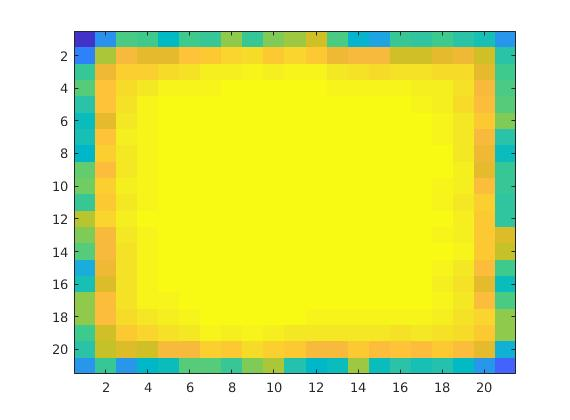
\includegraphics[width=1.3in]{pics/dat_gam_squ.jpg}}
\subfloat[]{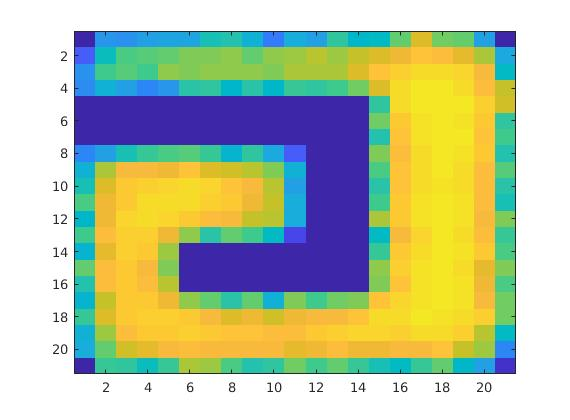
\includegraphics[width=1.3in]{pics/dat_gam_obs.jpg}}
\subfloat[]{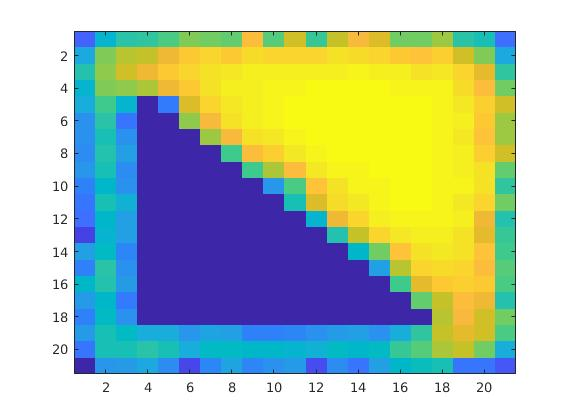
\includegraphics[width=1.3in]{pics/dat_gam_tri.jpg}}
\subfloat[]{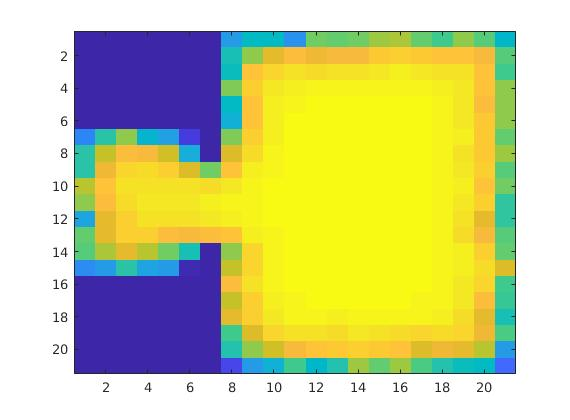
\includegraphics[width=1.3in]{pics/dat_gam_tbc.jpg}}
\caption{Value function of the various arenas for the agent aiming to purely maximise $\gamma$-empowerment. 
\textbf{(a)} is an empty arena. \textbf{(b)} is a snaking obstacle. \textbf{(c)} has a triangular obstacle with two corridors. \textbf{(d)} is an arena consisting of two rooms, where the agent initialises in the smaller room.\label{empfigs}
Here and in the following, agents were trained for $10^7$ episodes each of a length of 
twice the size of the environment with discount factor $\gamma=0.9$ and 
learning rate $\alpha=0.1$. 
For the single agent experiments the exploration rate was $\varepsilon=0.75$. 
	Yellow (blue) colour correspond to maximal (minimal) value at an 
arbitrary scale which is implied by the IRL scenario. 
	All values are non-negative. Inaccessible regions of the environment 
are assumed to have zero value.}
\end{figure}

\begin{figure}[!ht]
\centering
\subfloat[]{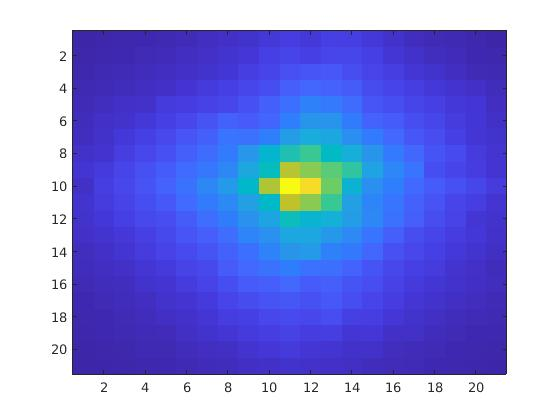
\includegraphics[width=1.3in]{pics/dat_comb_hi_squ.jpg}}
\subfloat[]{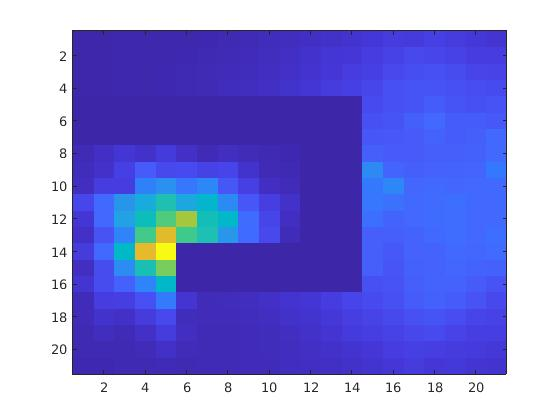
\includegraphics[width=1.3in]{pics/dat_comb_hi_obs.jpg}}
\subfloat[]{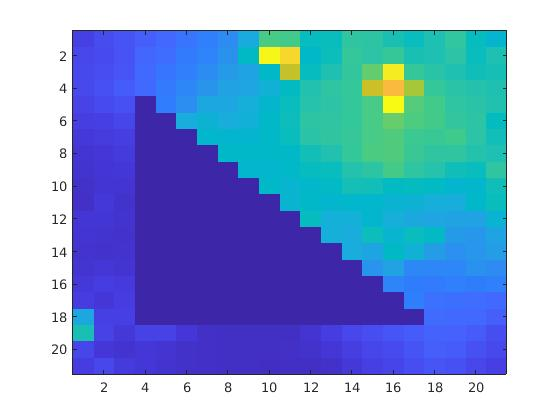
\includegraphics[width=1.3in]{pics/dat_comb_hi_tri.jpg}}
\subfloat[]{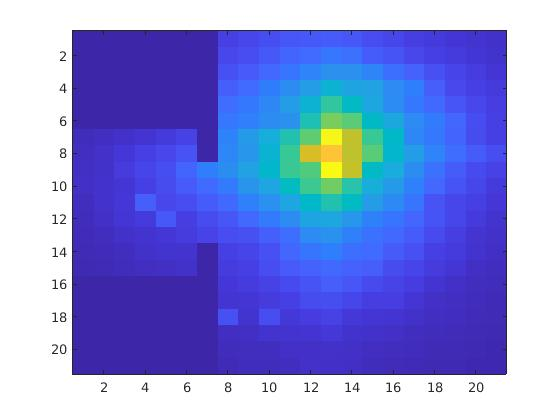
\includegraphics[width=1.3in]{pics/dat_comb_hi_tbc.jpg}}
\caption{Value function of the various arenas for the agents aiming to attempting to socialise. Agents are only rewarded for both choosing the action to greet the other within a Manhattan distance of 3. 
\textbf{(a)} is an empty arena. \textbf{(b)} is a snaking obstacle. \textbf{(c)} has a triangular obstacle with two corridors. \textbf{(d)} is an arena consisting of two rooms, where the agent initialises in the smaller room.\label{twohi}
Here and in the following, agents were trained for $10^7$ episodes each of a length of 
twice the size of the environment with discount factor $\gamma=0.9$ and 
learning rate $\alpha=0.1$, with $\varepsilon=0.5$.
	Yellow (blue) colour correspond to maximal (minimal) value at an 
arbitrary scale which is implied by the IRL scenario. 
	All values are non-negative. Inaccessible regions of the environment 
are assumed to have zero value.}
\end{figure}
\clearpage

\bibliographystyle{plainnat.bst}
\bibliography{bib_file}

\end{document}
